%-----------------------------------------------------------------------
%
\section{Examples}
\label{example}
%
%-----------------------------------------------------------------------

This section presents several examples to illustrate how the
implementation of the $\overline{\gamma}_{\alpha}-autotuning$
improves the performance of the closed-loop system respect to the
both operation modes.\\

In all the examples it is supposed that the process output can
vary in the 0 to 100\% normalized range and that in the normal
operation point, the controlled variable has a value close to
70\%. The corresponding system output to a 20\% set-point change
followed by a -20\% load-disturbance change are shown.

\subsection{Example 1}

Let us to consider the system (\ref{system_example}), shown before
as a \emph{Motivation Example}.\\

Table \ref{PID_parameters} shows the PID controller parameters for
the system (\ref{system_example}) using the
\cite{zhuangAthertonIEE1993} method and the proposed
$\overline{\gamma}_{\alpha}-autotuning$ with $\alpha=\{0.25, 0.50,
0.75\}$.\\

\begin{table}[h!]
\begin{center}
\caption{PID Controller Parameters}
\begin{tabular}{c|ccc}
\hline \textbf{tuning}               &$K_p$ &$T_i$ &$T_d$\\ \hline
$set-point(sp)$                               &1.66  &1.69  &0.51 \\
$load-disturbance(ld)$                        &2.42  &1.01  &0.56 \\
%$\gamma-autotuning$                           &1.98  &1.40  &0.53 \\
$\overline{\gamma}_{\alpha=0.25}-autotuning$  &1.79  &1.38  &0.52 \\
$\overline{\gamma}_{\alpha=0.50}-autotuning$  &1.95  &1.23  &0.53 \\
$\overline{\gamma}_{\alpha=0.75}-autotuning$  &2.02  &1.18  &0.53 \\
\hline
\end{tabular}
\label{PID_parameters}
\end{center}
\end{table}

System responses are shown in Fig. \ref{y_out} for the following
tuning methods: set-point, load-disturbance and
$\overline{\gamma}_{\alpha}-autotuning$ with its three possible
scenarios.\\

\begin{figure}[htb!]
    \begin{center}
        %\includegraphics[scale=0.8]{youtp.eps}
        \includegraphics[width=\linewidth]{youtp.eps}
        %\includegraphics[width=\linewidth]{y_outp.eps}
        \caption{Example 1, Process output for the control system operating in both servo and regulation modes}
        \label{y_out}
    \end{center}
\end{figure}

%\begin{figure}[htb!]
%    \begin{center}
%        \includegraphics[scale=0.8]{youtp1.eps}
%        %\includegraphics[width=\linewidth]{y_outp.eps}
%        \caption{: Example 1, Process output for the control system operating in both servo and regulation modes ($\alpha=0.25$)}
%        \label{y_out1}
%    \end{center}
%\end{figure}

%\begin{figure}[htb!]
%    \begin{center}
%        \includegraphics[scale=0.8]{youtp2.eps}
%        %\includegraphics[width=\linewidth]{y_outp.eps}
%        \caption{: Example 1, Process output for the control system operating in both servo and regulation modes ($\alpha=0.50$)}
%        \label{y_out2}
%    \end{center}
%\end{figure}

%\begin{figure}[htb!]
%    \begin{center}
%        \includegraphics[scale=0.8]{youtp3.eps}
%        %\includegraphics[width=\linewidth]{y_outp.eps}
%        \caption{: Example 1, Process output for the control system operating in both servo and regulation modes ($\alpha=0.75$)}
%        \label{y_out3}
%    \end{center}
%\end{figure}

It can be seen that the proposed
$\overline{\gamma}_{\alpha}-autotuning$ gives lower performance
than the optimum settings when the system operates in the same way
as it was tuned. However, higher performance can be obtained for
the whole system operation (regulatory-control and
servo-control), when an \emph{intermediate} controller is used.\\

Table \ref{values_PD} shows the Performance Degradation values
calculated from (\ref{PD_gamma_servo}) to (\ref{global_pd}) and
also the $WPD$ index (\ref{alpha_pd}) for each tuning. The below
side of the table presents the improvement in percentage that can
be achieved with each one of the
$\overline{\gamma}_{\alpha}-autotuning$ respect to the extreme
tunings (set-point and load-disturbance).\\

\begin{table}[h!]
\begin{center}
\caption{$PD$ and $WPD$ values for the system
(\ref{system_example}) and the improvement obtained with
$\overline{\gamma}_{\alpha}-autotuning$}
\begin{tabular}{c|cc|ccc}
\hline \textbf{tuning}       &$PD_{sp}$  &$PD_{ld}$ &$WPD_{\alpha=0.25}$ &$WPD_{\alpha=0.50}$ &$WPD_{\alpha=0.25}$\\
\hline
$set-point(sp)$                               &-          &0.3951 &0.0988 &0.1976 &0.2964\\
$load-disturbance(ld)$                        &0.9496     &-      &0.7123 &0.4748 &0.2374\\
%$\gamma-autotuning$                           &0.1129     &0.0534 &0.0980 & &\\
$\overline{\gamma}_{\alpha=0.25}-autotuning$  &0.0336     &0.1662 &0.0668 &- &-\\
$\overline{\gamma}_{\alpha=0.50}-autotuning$  &0.1088     &0.0376 &- &0.0732 &-\\
$\overline{\gamma}_{\alpha=0.75}-autotuning$  &0.1578     &0.0009 &- &- &0.0401\\
\hline \hline
improvement in \% of                          &            &            & & &\\
\hline
$\overline{\gamma}_{\alpha=0.25}-autotuning$  &96.46\%(ld) &57.93\%(sp) &32.39\%(sp) &- &-\\
                                              &            &            &90.34\%(ld) &- &-\\
$\overline{\gamma}_{\alpha=0.50}-autotuning$  &88.54\%(ld) &90.49\%(sp) &- &62.95\%(sp) &-\\
                                              &            &            &- &85.58\%(ld) &-\\
$\overline{\gamma}_{\alpha=0.75}-autotuning$  &83.38\%(ld) &99.77\%(sp) &- &- &86.47\%(sp)\\
                                              &            &            &- &- &83.11\%(ld)\\
(respect to)                                  &            &            & & &\\
\hline
\end{tabular}
\label{values_PD}
\end{center}
\end{table}

All the values confirm the fact that, in global terms, when both
operating modes could appear and taking into account the
percentage of the time that the control-loop is operating as servo
or regulation mode, the proposed
$\overline{\gamma}_{\alpha}-autotuning$ is the best choice to tune
the PID controller in order to get less Performance Degradations.

%\begin{table}[h!]
%\begin{center}
%\caption{$PD$ and $WPD$ values for the system
%(\ref{system_example}) and the improvement obtained with
%$\overline{\gamma}_{\alpha}-autotuning$}
%\begin{tabular}{c|ccc}
%\hline \textbf{tuning}       &$PD_{sp}$  &$PD_{ld}$ &$WPD$\\\hline
%$set-point(sp)$                               &-          &0.3951 &0.0988 \\
%$load-disturbance(ld)$                        &0.9496     &-      &0.7123 \\
%$\gamma-autotuning$                           &0.1129     &0.0534 &0.0980 \\
%$\overline{\gamma}_{\alpha=0.25}-autotuning$  &0.0336     &0.1662 &0.0668 \\
%\hline \hline
%improvement in \%                               &96.46\%(ld)       &57.93\%(sp)       &32.39\%(sp) \\
%of $\overline{\gamma}_{\alpha=0.25}-autotuning$ &70.24\%($\gamma$) &-2.11\%($\gamma$) &90.34\%(ld) \\
%(respect to)                                    &                  &                  &31.84\%($\gamma$) \\
%\hline
%\end{tabular}
%\label{values_PD1}
%\end{center}
%\end{table}

%\begin{table}[h!]
%\begin{center}
%\caption{$PD$ and $WPD$ values for the system
%(\ref{system_example}) and the improvement obtained with
%$\overline{\gamma}_{\alpha}-autotuning$}
%\begin{tabular}{c|ccc}
%\hline \textbf{tuning}       &$PD_{sp}$  &$PD_{ld}$ &$WPD$\\\hline
%$set-point(sp)$                               &-          &0.3951 &0.1976 \\
%$load-disturbance(ld)$                        &0.9496     &-      &0.4748 \\
%$\gamma-autotuning$                           &0.1129     &0.0534 &0.0832 \\
%$\overline{\gamma}_{\alpha=0.50}-autotuning$  &0.1088     &0.0376 &0.0732 \\
%\hline \hline
%improvement in \%                               &88.54\%(ld)       &90.49\%(sp)       &62.95\%(sp) \\
%of $\overline{\gamma}_{\alpha=0.50}-autotuning$ & 3.65\%($\gamma$) &29.64\%($\gamma$) &84.58\%(ld) \\
%(respect to)                                    &                  &                  &12.02\%($\gamma$) \\
%\hline
%\end{tabular}
%\label{values_PD2}
%\end{center}
%\end{table}

%\begin{table}[h!]
%\begin{center}
%\caption{$PD$ and $WPD$ values for the system
%(\ref{system_example}) and the improvement obtained with
%$\overline{\gamma}_{\alpha}-autotuning$}
%\begin{tabular}{c|ccc}
%\hline \textbf{tuning}       &$PD_{sp}$  &$PD_{ld}$ &$WPD$\\\hline
%$set-point(sp)$                               &-          &0.3951 &0.2964 \\
%$load-disturbance(ld)$                        &0.9496     &-      &0.2374 \\
%$\gamma-autotuning$                           &0.1129     &0.0534 &0.0683 \\
%$\overline{\gamma}_{\alpha=0.75}-autotuning$  &0.1578     &0.0009 &0.0401 \\
%\hline \hline
%improvement in \%                               &83.38\%(ld)       &99.77\%(sp)       &86.47\%(sp) \\
%of $\overline{\gamma}_{\alpha=0.75}-autotuning$&-39.77\%($\gamma$) &98.31\%($\gamma$) &83.11\%(ld) \\
%(respect to)                                    &                  &                  &41.29\%($\gamma$) \\
%\hline
%\end{tabular}
%\label{values_PD3}
%\end{center}
%\end{table}


%------------------------------------
%
\subsection{Example 2}
%
%------------------------------------

In order to add completeness to the comparison, a second example
is introduced. The problem of control a
Continuous-Stirred-Tank-Reactor (CSTR) as the one in Fig.
\ref{CSTR} with the numerical values taken from \cite{Huang96}.\\

\begin{figure}[htb!]  \label{fig:cstr}
\centering
\includegraphics[width=0.5\linewidth]{Reactor01.eps}
\caption{CSTR System} \label{CSTR}
\end{figure}

The goal is to control the reactor composition by manipulating the
cool rate through the control signal $u$. The transfer function of
the system has the form

\be P_2(s)=\frac{-1.308 e^{-4.896s}}{(13.515s+1)(6.241s+1)} \ee

In order to put more relevance to the control-loop operation
issue, a First-Order-Plus-Dead-Time approximation is computed with
$K_p=-1.3$, $T=16$ and $L=9.5$. The proposed
$\overline{\gamma}_{\alpha}-autotuning$ with $\alpha=0.50$, the
$\gamma-autotuning$, as well as the extreme tunings for set-point
and load-disturbance are used on the basis of this model
information. The parameters for the controller are in Table
\ref{PID_parameters2}.

\begin{table}[h!]
\begin{center}
\caption{PID Controller Parameters for CSTR System}
\begin{tabular}{c|ccc}
\hline \textbf{tuning}                        &$K_p$  &$T_i$ &$T_d$\\
\hline
$set-point(sp)$                               &-1.29  &16.39  &4.92 \\
$load-disturbance(ld)$                        &-1.88  & 9.69  &5.37 \\
$\gamma-autotuning$                           &-1.54  &13.50  &5.12 \\
%$\overline{\gamma}_{\alpha=0.25}-autotuning$ & 1.79  & 1.38  &0.52 \\
$\overline{\gamma}_{\alpha=0.50}-autotuning$  &-1.51  &11.89  &5.06 \\
%$\overline{\gamma}_{\alpha=0.75}-autotuning$ & 2.02  & 1.18  &0.53 \\
\hline
\end{tabular}
\label{PID_parameters2}
\end{center}
\end{table}

Fig. \ref{example2_fig2} shows the output responses. Once again,
it can be seen that both, the proposed
$\overline{\gamma}_{\alpha}-autotuning$ and $\gamma-autotuning$,
give lower performance than the optimal settings when the system
operates in the same way as it was tuned, but considering that
set-point changes as well as load-disturbances can appear in a
realistic control system, the global performance is better for the
\emph{intermediate} tunings.\\

If we look the data in Table \ref{values_PDCSTR} it can be seen
that the proposed $\overline{\gamma}_{\alpha}-autotuning$ method,
even providing slightly lower degradation, achieves good
improvement indices.

\begin{figure}[htb!]
\centering
\includegraphics[width=\linewidth]{CSTR_output}
\caption{Example 2, CSTR Control System output}
\label{example2_fig2}
\end{figure}

\begin{table}[h!]
\begin{center}
\caption{$PD$ and $WPD$ values for the CSTR system and the
improvement obtained with $\overline{\gamma}_{\alpha}-autotuning$}
\begin{tabular}{c|ccc}
\hline \textbf{tuning}                        &$PD_{sp}$  &$PD_{ld}$ &$WPD_{\alpha=0.50}$\\
\hline
$set-point(sp)$                               &-          &0.3979    &0.1990 \\
$load-disturbance(ld)$                        &0.9642     &-         &0.4821 \\
$\gamma-autotuning$                           &0.1143     &0.0533    &0.0838 \\
$\overline{\gamma}_{\alpha=0.50}-autotuning$  &0.1097     &0.0373    &0.0735 \\
\hline \hline
improvement in \% of                         &88.62\%(ld)       &90.63\%(sp)       &63.07\%(sp) \\
$\overline{\gamma}_{\alpha=0.50}-autotuning$ & 4.02\%($\gamma$) &30.02\%($\gamma$) &84.75\%(ld) \\
(respect to)                                 &                  &                  &12.29\%($\gamma$) \\
\hline
\end{tabular}
\label{values_PDCSTR}
\end{center}
\end{table}
